\subsection{Automating data processing}
An end-to-end computational workflow was developed for data quality
improvement to address the reported data quality issue.

\subsubsection{Data staging and processing environment}
Raw data from all ARM instruments are versioned and saved in deep
archive on the High Performance Storage System (HPSS) \cite{Watson_HSI_2005}
at Oak Ridge Leadership Computing Facility \cite{olcf_hpss}. An
automated process was developed to query the database for any data
quality issue iand based on it's unique DQR ID, identify all raw data files
impacted by the reported issues; the impacted datasets are then
retrieved from the archive. Two different
methods for data retrieval were implemented: 1) automated retrievals
using HPSS Hierarchical Storage Interface (HSI) \cite{Watson_HSI_2005}
which can be used across
most of the computational systems within ARM Data Center, but,
performs a sequential retrieval of files; and 2) a Globus Online
\cite{Foster_Globus_2011,Allen_SSD_2012} based
fast and parallel transfer mechanism suitable for large volumes of data.  

\subsubsection{Instrument data dictionaries}
Raw data from each individual instrument, which number in hundreds across
ARM facility, are all often different depending on sensors, data
characteristics and manufacturers. The raw data format ranges from space or comma
separated ASCII, binary, hex etc. Ability to automate the processing of
datasets require a good machine readable metadata and descriptors for
each instrument. Traditional processing workflows were custom
designed for individual instruments and thus lead to rigid workflow that
required custom developments to address any quality issues. As part of
automated workflow, detailed data dictionaries were designed and saved
in machine readable JSON formats that allowed for automated processing
of data. Data dictionary encodes the format of raw instrument data,
numerical procedure to calculated derived variables, and ARM standard
variable names and units (Figure~\ref{fig:met_dict}). Data dictionaries
also capture any historical change or update to instrument data format
or observations. Figure~\ref{fig:met_dict} shows an example data
dictionary for surface meteorology (MET) instruments the contains the
column-wise mapping of data in raw ASCII format, expected data type,
units and names for standard primary and derived variables.
Library of comprehensive data dictionaries are the
critical to enable automation of data quality control and improvements
at scale across large observational facility like ARM. 

\begin{figure}
 \centering
 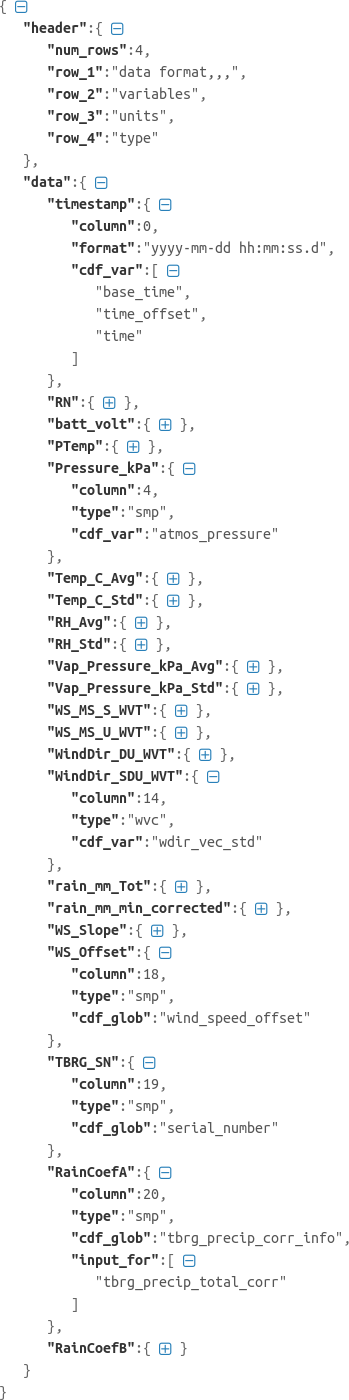
\includegraphics[width=0.6\linewidth]{figures/met_dict.png}
 \caption{Data dictionary for MET instrument contains information about
	 the raw data format, standard variable names, units, variable dependencies
	 and other metadata in a JSON format.}
 \label{fig:met_dict}
\end{figure}

\subsubsection{Symbolic equations processing}
As part of automated data processing framework, a capability for
symbolic equation processing was developed using Python \texttt{SymPy}
\cite{sympy}. Equations for calculating any primary or derived variables are
derived from instrument data dictionaries or provided by instrument
experts as part of the associated DQR. Equations provided with DQRs are
given precedence over ones from data dictionaries. Framework was
designed to ensure the correctness of associated variables to be
processed for any given data stream. When solving system or set of
equations, the framework was designed to detect and handle and variable
dependence and/or conflict. If primary variable is changed as part of
a data quality issue, all dependent derived variables were recalculated
to ensure correctness of the entire data stream as part of the processing.
Framework was implemented and tested for a range of scenarios experienced
within ARM datasets for correctness and accuracy before being deployed
operationally. Ability to process symbolic equations allowed for automation of data
improvement workflow, avoid need for any custom development and
processing by an analyst.

\subsubsection{High performance computing for big data processing}
For efficient processing of large volumes of data, capability for
parallel data processing was developed. Most ARM time series data are
packaged in one or more files per day allowing for their simultaneous
processing in a embarrassingly parallel fashion. Two parallel processing
framework were implemented within the Python based software framework,
to allow for use and execution on small shared memory computing
environment to medium to large scale distributed memory computing
environments. For shared memory environment, parallelism was achieved
using Python \texttt{multiprocessing} while Python \texttt{Dask}
\cite{dask} was used for parallel data processing on distributed memory
compute clusters. For task requiring processing for large volume of
data, data transfers times are significant and system was designed to
overlap data staging and processing to allow processing of data as soon
as they
become available.

\subsubsection{Data review}
Review of the processing performed on the data is critical to ensure
that the actions undertaken accurately and satisfactorily addressed the
data quality issues reported in the associated DQR.
A formal and comprehensive data review was conducted for each corrected
and processed datasets,
comparing old and new data products to identify variables
affected, compute statistics for change and generate interactive plots
to visualize the data. Data review was one of the only step that was
designed to require a human intervention, in form of review either by
the instrument expert or the data analyst. While the workflow was
designed for automation, the free-form description section of the DQR
may at times contain special instructions or information that may have been missed by the
automation workflow. Data review was designed to provide the oversight
to ensure the accuracy of the data. If the data review check is
successful, it triggers the execution of the rest of the workflow,
however in case an issue is identified the processing task is
assigned to a data analyst. 




